%%
%% This is file `./samples/longsample.tex',
%% generated with the docstrip utility.
%%
%% The original source files were:
%%
%% apa7.dtx  (with options: `longsample')
%% ----------------------------------------------------------------------
%% 
%% apa7 - A LaTeX class for formatting documents in compliance with the
%% American Psychological Association's Publication Manual, 7th edition
%% 
%% Copyright (C) 2021 by Daniel A. Weiss <daniel.weiss.led at gmail.com>
%% 
%% This work may be distributed and/or modified under the
%% conditions of the LaTeX Project Public License (LPPL), either
%% version 1.3c of this license or (at your option) any later
%% version.  The latest version of this license is in the file:
%% 
%% http://www.latex-project.org/lppl.txt
%% 
%% Users may freely modify these files without permission, as long as the
%% copyright line and this statement are maintained intact.
%% 
%% This work is not endorsed by, affiliated with, or probably even known
%% by, the American Psychological Association.
%% 
%% ----------------------------------------------------------------------
%% 
\documentclass[man]{apa7}

\usepackage{lipsum}

\usepackage[american]{babel}

\usepackage{caption} % For captioning outside figures
\usepackage{capt-of} % For captioning outside figures

\usepackage{siunitx}

\usepackage{csquotes}
\usepackage[style=apa,backend=biber]{biblatex}
\addbibresource{bibliography.bib}

\title{Laser Scanning Comparison Using CloudCompare}
\shorttitle{}
\authorsnames{Jule Valendo Halim -1425567}
\authorsaffiliations{GEOM90038 - Advanced Imaging}

\begin{document}

\maketitle
\tableofcontents
\newpage
\section{Introduction}
\vspace{-5em}
Light detection and ranging (LiDAR) sensor consists of a transmitter and a receiver. The transmitter contains a laser that emits beams of light, while the receiver collects the photons that return from the transmitted laser (\Textcite{wandinger2005}). Figure \ref{fig:lidarSetup} shows a simple representation of a LiDAR system.

\begin{minipage}{\linewidth}
  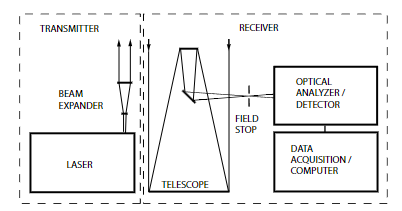
\includegraphics[bb=0in 0in 2.5in 2.5in, height=2.5in, width=2.5in]{figures/lidarSetup.png}
  \captionof{figure}{Principle setup of a LiDAR system (\Textcite{wandinger2005})}
  \label{fig:lidarSetup}
\end{minipage}

Multiple forms of LiDAR systems can be used for various applications. For example, \Textcite{conti2024} compared two applications of LiDAR sensors in the use of an Italian town hall building. The two sensor applications are terrestrial and mobile laser scanners (TLS and MLS respectively). A terrestrial laser scanner uses a LiDAR sensor mounted on a tripod and scans the area around it. The TLS is able to capture a wide area through a mirror within the hardware that can rotate and reflect the lasers in many angles. Meanwhile, the MLS is a handheld LiDAR sensor that can be carried and transported with one hand. Capturing wider areas with this device is possible due to the handheld nature, where a user would move around and capture the entire area. Figure \ref{fig:TLSandMLS} shows a MLS and TLS device.

\begin{minipage}{\linewidth}
  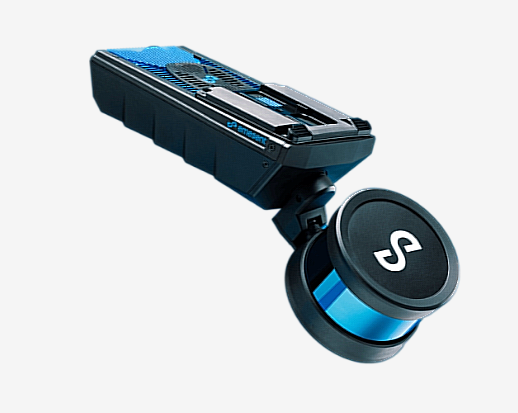
\includegraphics[height=\textheight/3,width=\textwidth/2]{figures/HoverMap.png}
  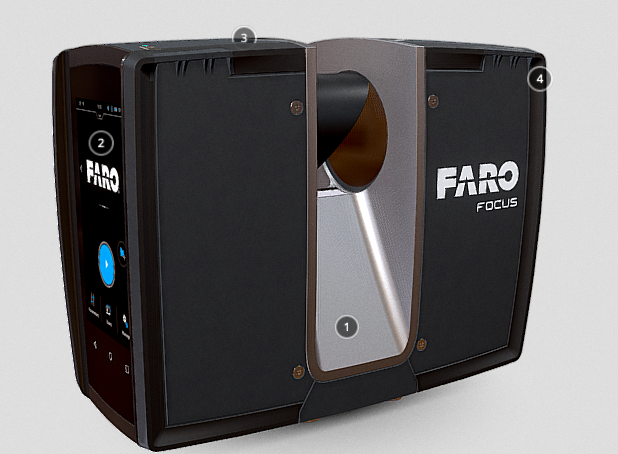
\includegraphics[height=\textheight/3,width=\textwidth/2]{figures/FaroFocus.png}
  \captionof{figure}{Hovermap Emesent MLS (left) (\Textcite{emesent}) and FAROFocus TLS (right) (\Textcite{FARO})}
  \label{fig:TLSandMLS}
\end{minipage}

\Textcite{conti2024} found that the MLS is able to create a streamlined and efficient workflow that is suitable for the documentation of heritage buildings. However, where a higher level of detail is required, the TLS would be more suitable. In this report, I aim to investigate the differences in the MLS and TLS through using the LiDAR systems shown in figure 2. Dense point clouds will be obtained for each system before being compared using the open source software CloudCompare (\Textcite{cloudcomparesoftware}). This software has been shown to be able to compare two different point clouds and investigate their respective quality (\Textcite{girardeau2016}). 

The overall procedure in investigating both LiDAR systems involves with firstly determining hardware settings and object to be scanned, followed by performing the scan to create a dense point cloud. The resulting point clouds will then be aligned and compared to each other qualitative and quantitatively. More details regarding the project procedure will be discussed in the methods section.
\newpage
\section{Method}

\subsection{Initial Settings and Point Cloud Capturing}

The building chosen was a room in the University of Melbourne Building 207-221 Bouverie St. For the remainder of the report, the MLS will refer to the Hovermap Emesent and the TLS will refer to the FAROFocus.

Initial settings were set to capture an indoor area with a range of 10m (ie., the room boundaries are within 10m of the TLS). The TLS was also configured to capture images using colour. Afterwards, the resolution and quality settings are set to 1/5 and 4x respectively. The resolution indicates that one in every 5 points would be scanned, and the quality indicates that each of these scans would occur 4 times. Additional setting for the TLS such as the pixel dimensions of each scan and time taken for the scan can be seen in figure \ref{fig:TLSSettings}. A scan was then executed with these settings.

\begin{minipage}{\linewidth}
  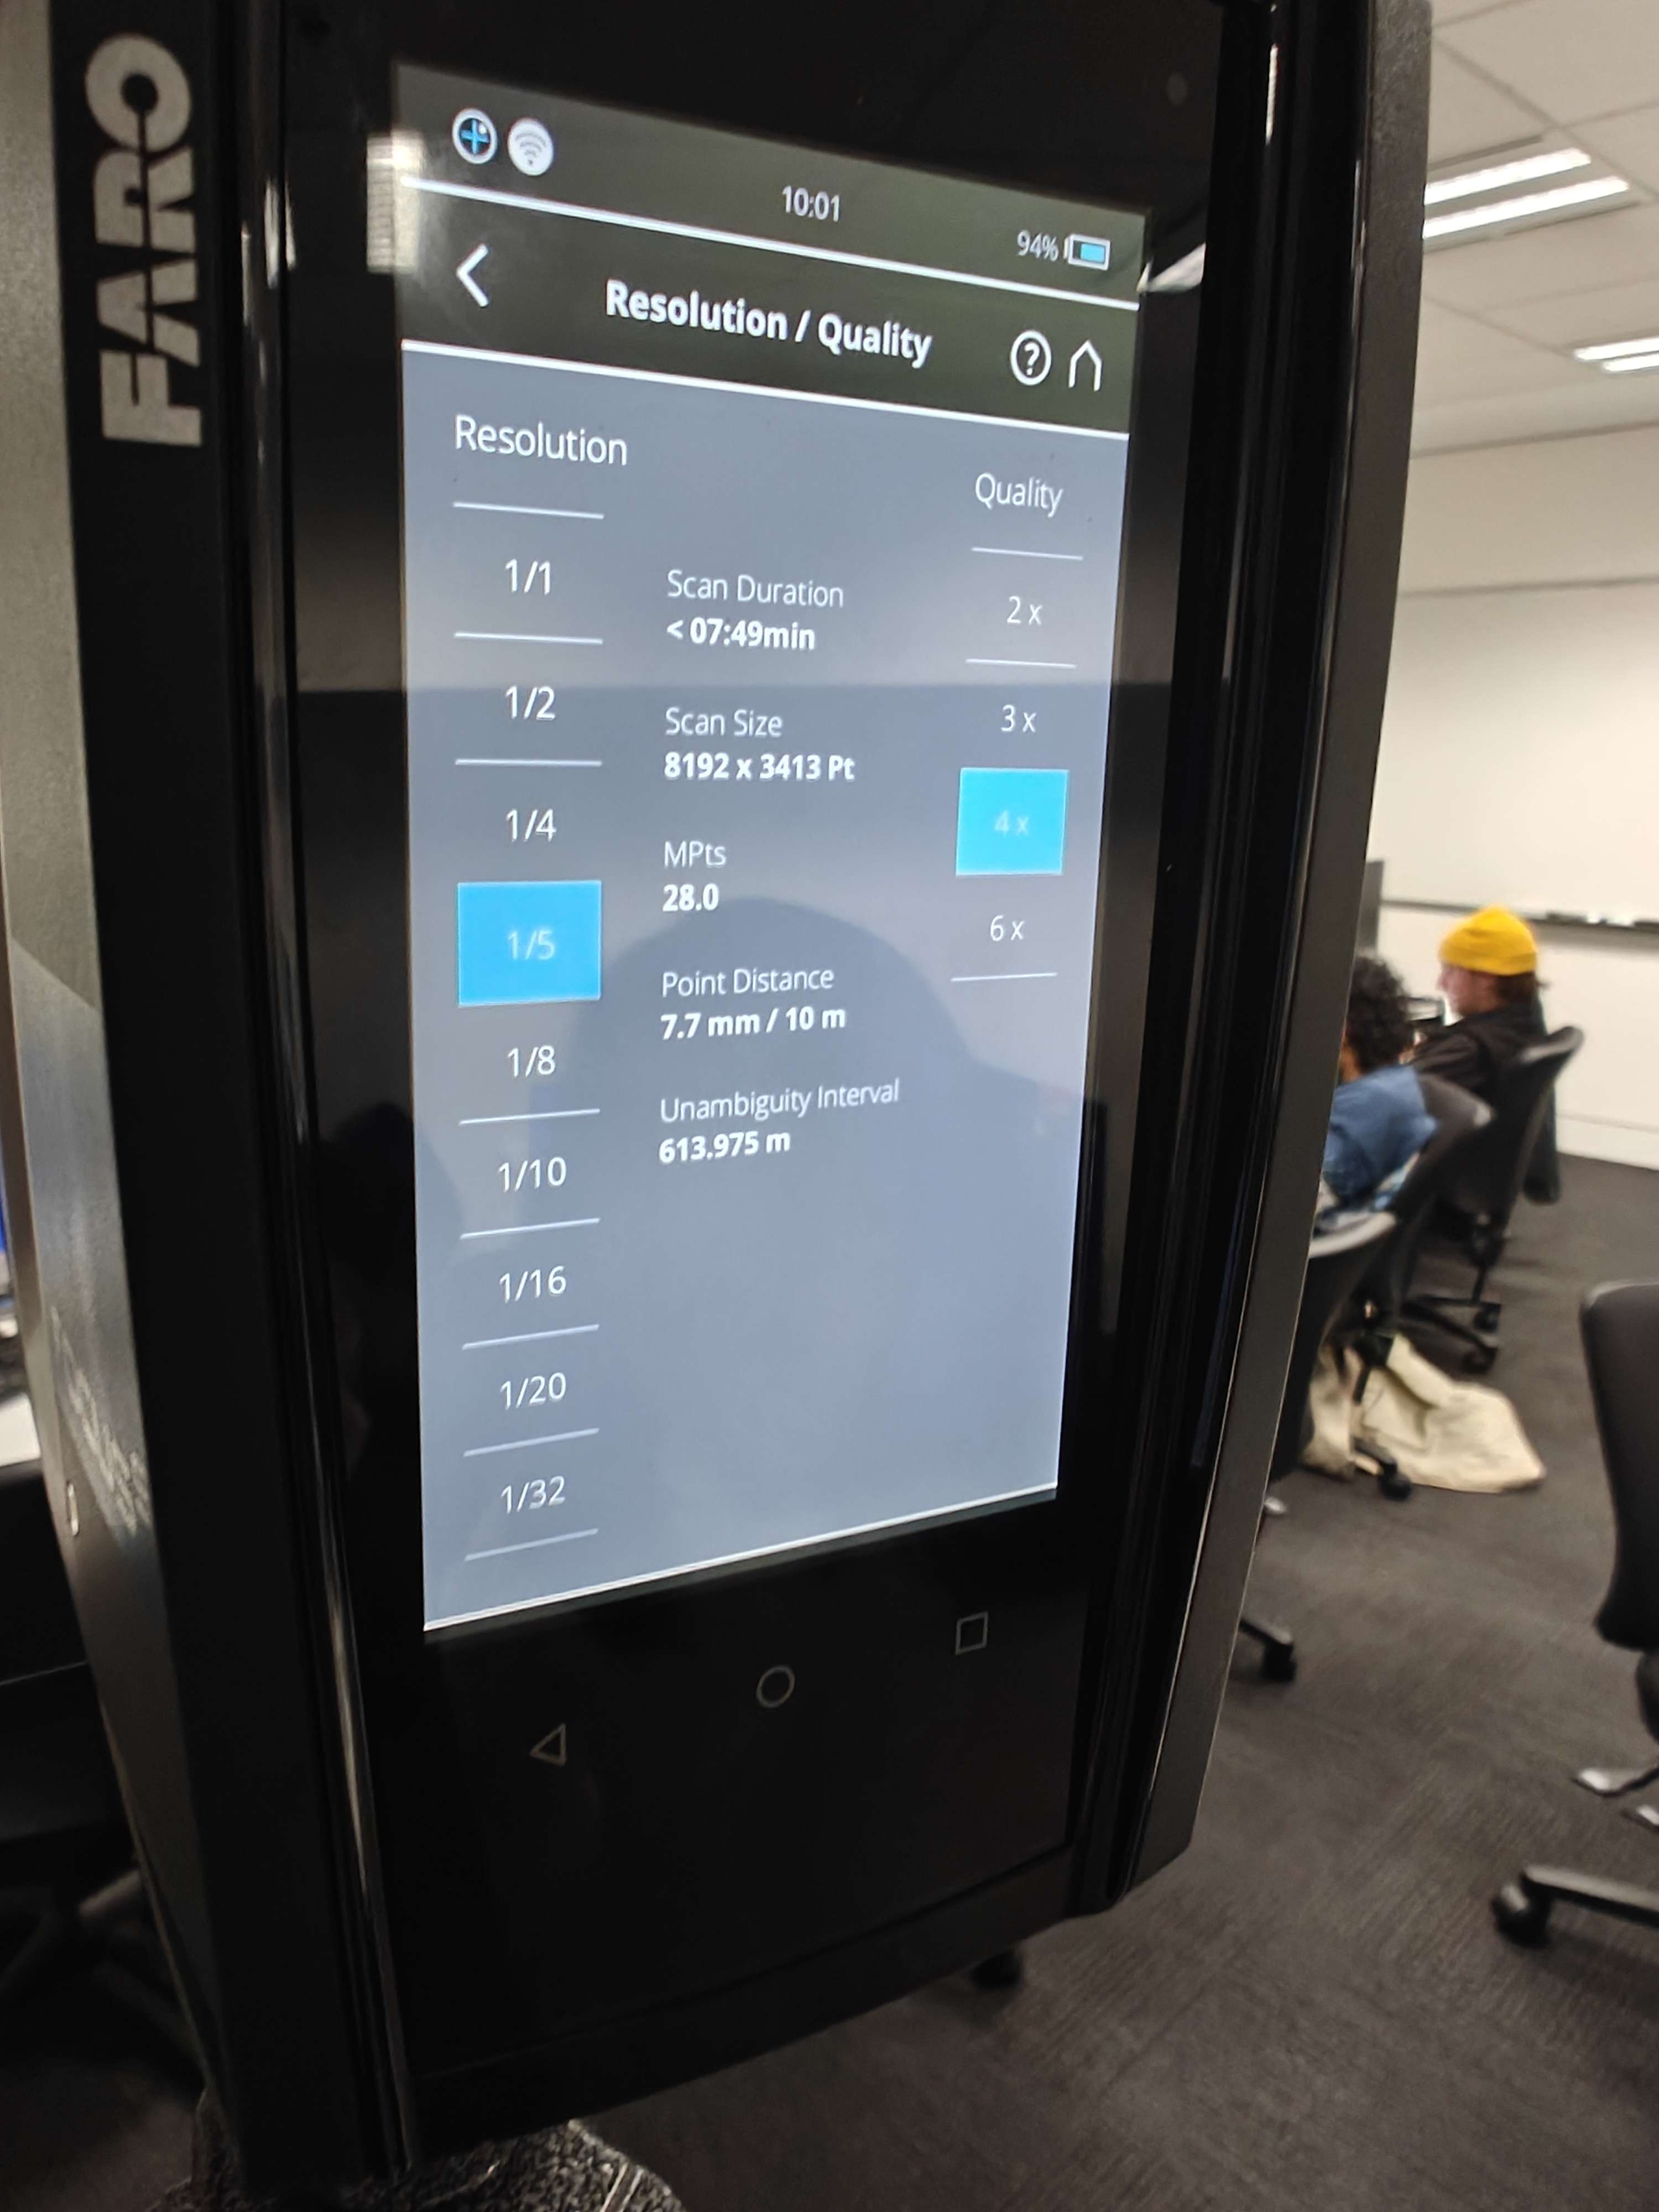
\includegraphics[height=\textheight/3 ,width=\textwidth/3]{figures/IMG20240418194000.jpg}
  \captionof{figure}{Settings for the TLS}
  \label{fig:TLSSettings}
\end{minipage}

The MLS was first connected to its mobile app. After this connection is established, the app can be used to control its operation (ie., starting and stopping its scan). The MLS was moved around the room and for each area, the MLS was held for a few seconds to ensure that it could capture the entire area. Places where might not be captured by the MLS easily (e.g., under a table or an object that is high on the walls) would be further scanned using different angles.


\subsection{TLS and MLS Point Cloud Alignment}

\subsubsection{Manual Alignment}
Both point clouds were added to the CloudCompare working space. Using the rotation and trasnlation tools, the MLS point cloud was carefully oriented to overlap with the orientation and position in space of the TLS. Figure \ref{fig:manualAlignment} shows the difference of orientation after manual alignment. The grey point clouds are from the MLS, while the point cloud with more colour is from the TLS.

\begin{minipage}{\linewidth}
  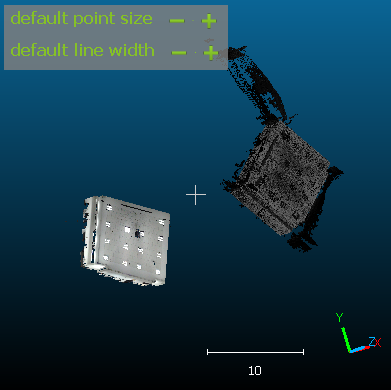
\includegraphics[height=\textheight/3,width=\textwidth/2]{figures/InitialAlignments.png}
  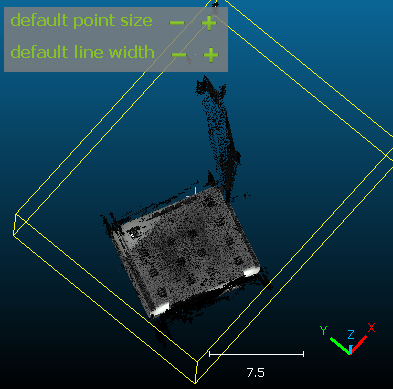
\includegraphics[height=\textheight/3,width=\textwidth/2]{figures/FinalAlignments.png}
  \captionof{figure}{Inital alignments when point clouds were added (left) and the result of manual alignment (right)}
  \label{fig:manualAlignment}
\end{minipage}

Visual inspection was done at this stage to identify whether or not each point cloud appeared to be aligned. Afterwards, coarse and fine registration was used to identify the errors in alignment.

\subsubsection{Coarse and Fine Registrations}
Coarse registration is done by using the align (point pairs picking) tool in CloudCompare. This tool performs references one point cloud to the other using reference points selected manually. A total of 6 (3 in each point cloud) reference points were selected. The MLS is the to-be-aligned entity, while the TLS was the reference point cloud. Figure \ref{fig:roughAlignment} shows the coordinates and positions of the 7 pairs of reference points selected. The total RMS is also shown in the same image.

\begin{minipage}{\linewidth}
  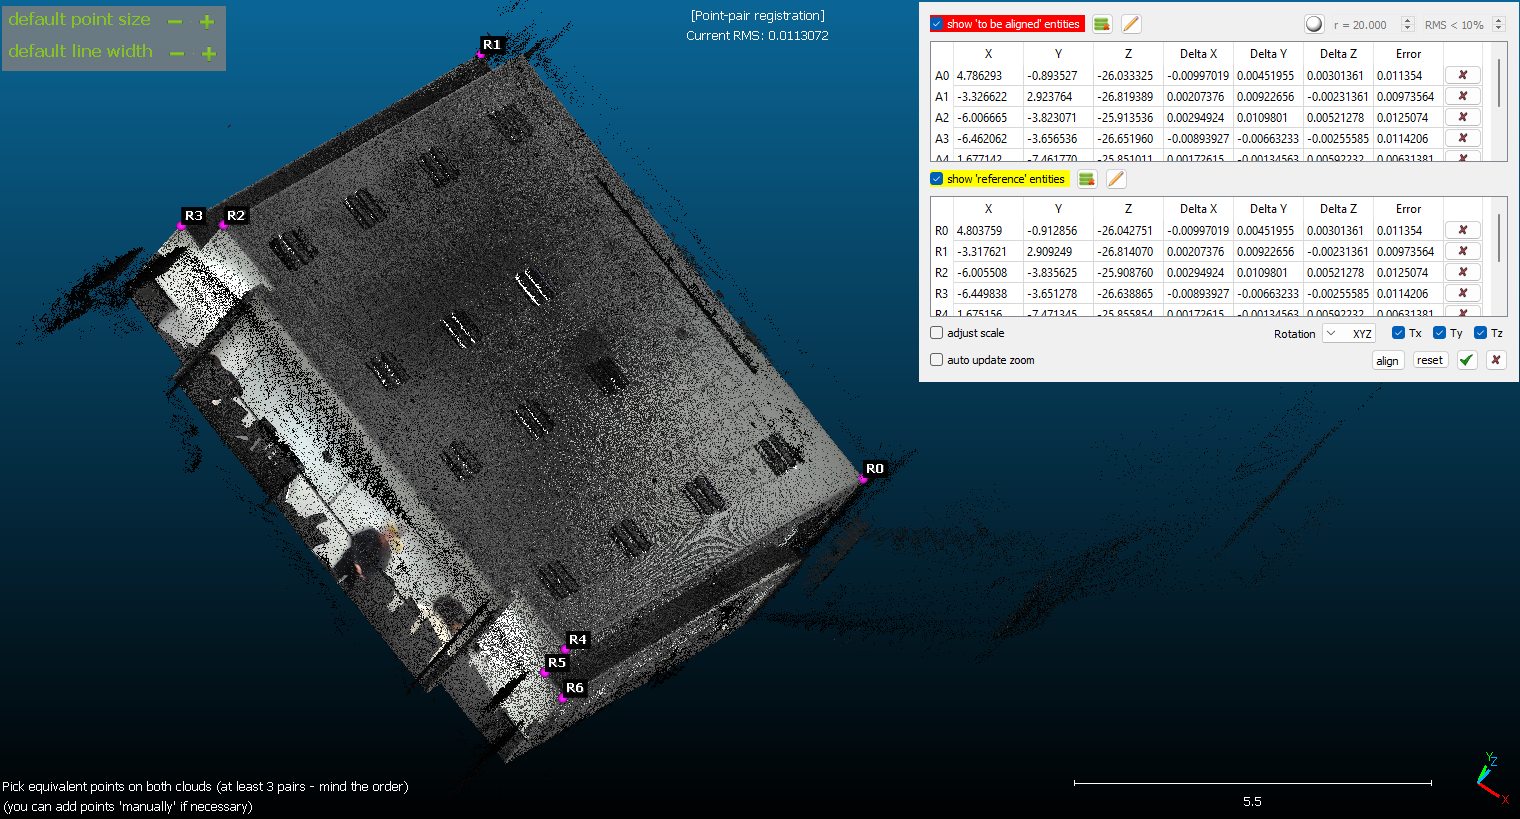
\includegraphics[height=200px,width=450px]{figures/RoughAlignment1.png}
  \captionof{figure}{Rough Alignment Showing the Points Used for Referencing}
  \label{fig:roughAlignment}
\end{minipage}

Afterwards, fine registration was performed. This process involved using the fine registration (ICP) tool from CloudCompare. Fine registration is only done after coarse registration. Again, the TLS was the reference point and the MLS was the reference point cloud. For both registrations, the registration errors (RMSE) (in meters) and transformation matrices were recorded after registration was completed.

\subsection{Cloud to Cloud Distance}

Cloud to cloud distances were then calculated using the Cloud-Cloud Dist tool. This tool calculates the distances from the points present in each cloud. Initally, there was no maximum distance placed this distance to distance calculation. This was done in order to identify what areas have high distances. Figure \ref{fig:nomaxdistance} shows the cloud to cloud distance without any maximum distance. 


Investigating this distance map showed that most of the areas where the point clouds are overlapping have very small distances (most were less than 1.9m), and that the RMSEs obtained from registration was approximately 0.2m, the maximum distance was set at 1m in order to obtain a clearer view of where the errors come from. Higher maximums were also tested (such as 4m and 8m). However, these proved to be not very informative as the entire overlapping area only had one colour.

\begin{minipage}{\linewidth}
  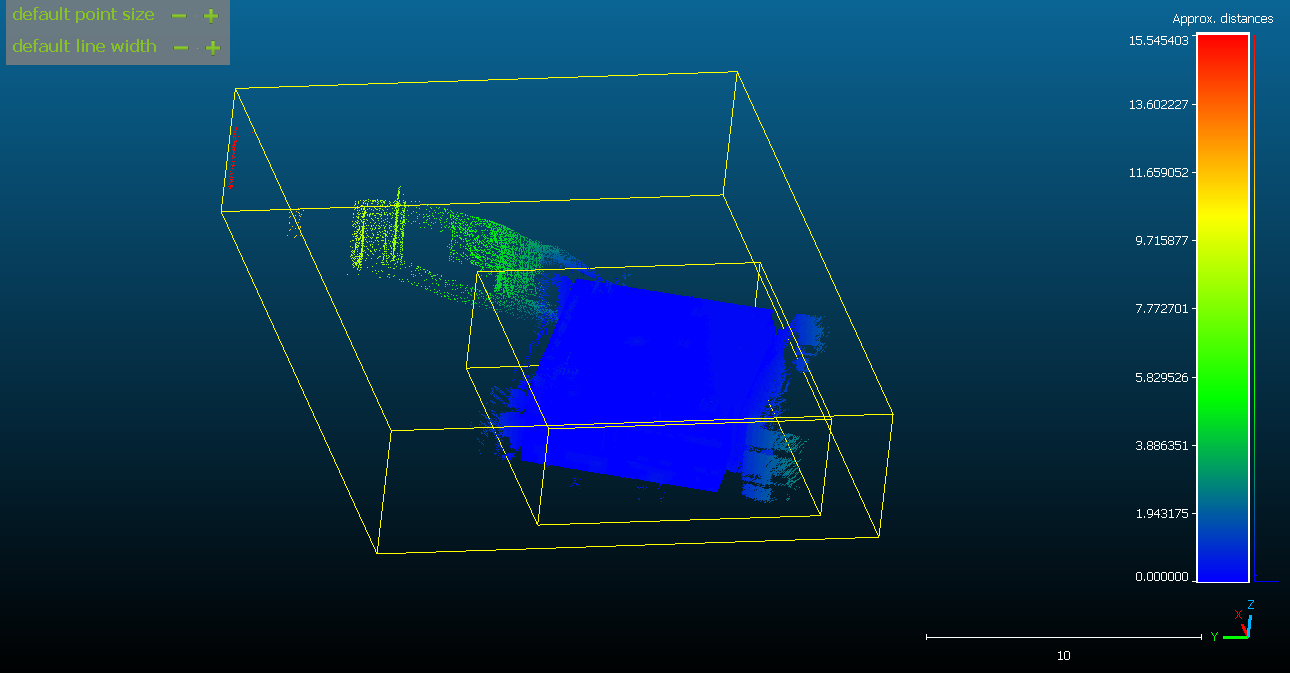
\includegraphics[height=\textheight/2 ,width=\textwidth/1]{figures/noMaxDistance.png}
  \captionof{figure}{Cloud to Cloud Distance Without Maximum Distance}
  \label{fig:nomaxdistance}
\end{minipage}

After cloud to cloud distances were obtained and visualized, the TLS and MLS point clouds were exported as text files for further analysis in the results section. 
\newpage
\section{Results and Analysis}

\subsection{Registration Errors}

RMSE and transformation matrices for coarse and fine registrations are shown in figures \ref{fig:rmsecoarsefine}.

\begin{minipage}{\linewidth}
  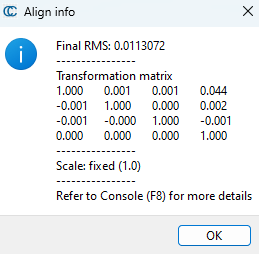
\includegraphics[height=\textheight/4 ,width=\textwidth/3]{figures/RoughAlignment2.png}
  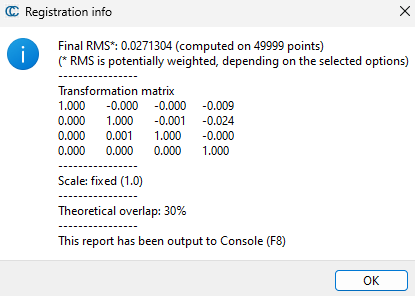
\includegraphics[height=\textheight/4 ,width=\textwidth/2]{figures/FairAlignment1-30_.png}
  \captionof{figure}{RMSE and Transformation Matrices for Coarse (left) and Fine (right) Registration}
  \label{fig:rmsecoarsefine}
\end{minipage}

Theoretical overlap is a parameter that is used in fine registration to indicate how many percent of the points are expected to overlap from one another. Multiple values ranging from 10-100\% were tested. However, 30\% was selected as the final value in order to reduce the final RMS.

The RMS values show great accuracy, with the coarse registration having an RMS of 1.13cm while the fine registration has 2.27cm of final RMS values.


\subsection{Cloud to Cloud Distance Results}

The full C2C distances consists of millions of points, and so will be omitted from this report. The means and standard deviations of C2C distances are shown in table \ref{tab:RMStable}. All three statistical measures were shown for the set of distances calulated for all point clouds, for the section where only distances less than or equal to 1 were kept, and sections where distances were greater than 1.

\begin{minipage}{\linewidth}
  \small
  \captionof{table}{Table Showing Statistical Information About C2C Distances}
  \setlength{\tabcolsep}{3pt} % reduce column spacing
  \renewcommand{\arraystretch}{0.8} % reduce row spacing
  \label{tab:RMStable}
  \begin{tabular}{@{}llrr@{}}         \toprule
  \multicolumn{4}{c}{C2C Distance Statistics }        \\ \toprule{}
  &  All Distances|    & Distances <= 1m| & Distances > 1m \\ \midrule
  Number of Points & 30,663,458  & 30,640,551  & 22,907  \\
  \% of Total Points (rounded to 2 significant figures) & 100\% & 99.93\% & 0.00075\% \\
  Mean (m)      & 0.091 & 0.090 & 2.349  \\
  Median (m)    & 0.039 &  0.039  & 1.425   \\
  Maximum Value (m)       & 15.575  & 0.99998  & 15.575   \\
  Minimum Value (m)       & \num{1.4e-05}  & \num{1.4e-05} & 1.000001  \\
  Standard Deviation (m)  & 0.162  & 0.139 & 2.141 \\ 
  Approximate Max Error(m) \footnote{Max error was calcualted using CloudCompare, which only allows a setting of maximum distance, not minumum distance. As such, distances less than 1 was possible through the use of iteratively subsectioning and checking the maximum distance until the max distance was approximately 1, and then running a distance computation. This is not possible to be done with distances greater than 1. A through description of this proccess is found in Appendix A.} & 0.09 &  0.046 & N/A \\ \bottomrule
  \end{tabular}
\end{minipage}

Figure \ref{fig:nomaxdistance} above shows the spatial distribution of errors with no maximum limit while figure \ref{fig:maxdistanceset} shows the distribution of distances with C2C distances less than 1.

\begin{minipage}{\linewidth}
  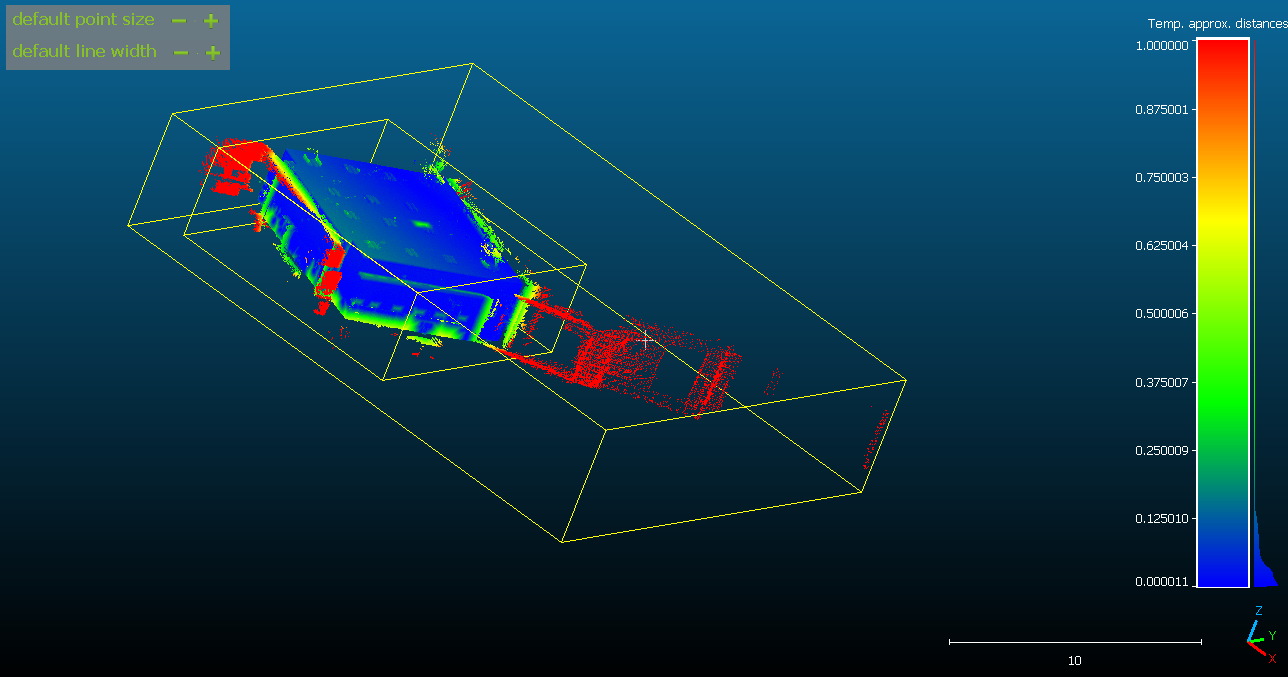
\includegraphics[height=\textheight/4 ,width=\textwidth/2]{figures/DistanceModel2.png}
  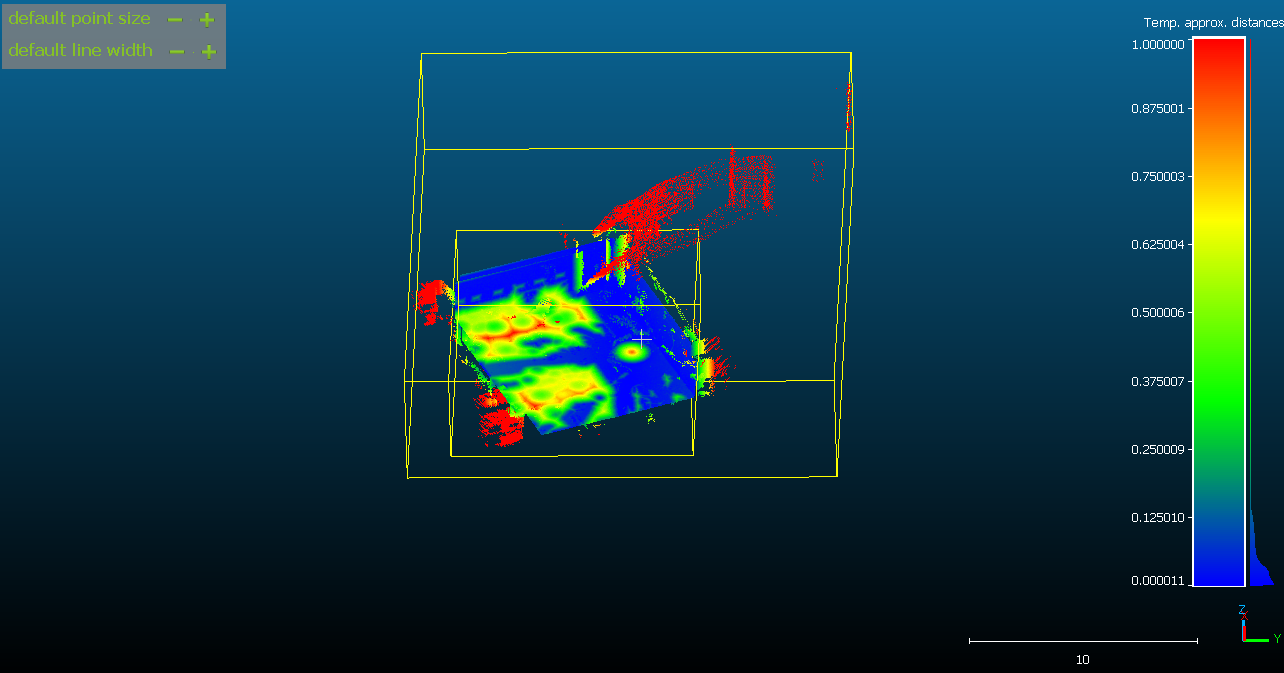
\includegraphics[height=\textheight/4 ,width=\textwidth/2]{figures/DistanceModel.png}
  \captionof{figure}{Spatial Distribution of C2C Distances From Above (left) and Below (right) for Distances Less than 1}
  \label{fig:maxdistanceset}
\end{minipage}

\newpage

As seen in figures \ref{fig:manualAlignment}, \ref{fig:nomaxdistance}, and \ref{fig:maxdistanceset}, most of the TLS and MLS point clouds have a significant amount of overlap. However, there are still some areas in which the MLS deviates from the TLS point cloud. Particularly, the areas in figure  \ref{fig:maxdistanceset} where the point clouds are red. This indicates that they have a high amount of C2C distances.

To study only the overlapping areas, the MLS acted as the reference point cloud for the TLS. This would ensure that only points that are in both TLS and MLS are being investigated, as the TLS has been shown to be a subset of the MLS (figure \ref{fig:maxdistanceset}). Table \ref{tab:RMStable2} shows the statistical information regarding C2C distances where the MLS was acting as the reference point cloud. 

\vspace{2em}

\begin{minipage}{\linewidth}
  \small
  \captionof{table}{Table Showing Statistical Information About C2C Distances with MLS as the Reference Point Cloud}
  \setlength{\tabcolsep}{3pt} % reduce column spacing
  \renewcommand{\arraystretch}{0.8} % reduce row spacing
  \label{tab:RMStable2}
  \begin{tabular}{@{}llrr@{}}         \toprule
  \multicolumn{2}{c}{C2C Distance Statistics }        \\ \toprule{}
  &  MLS as Reference Point Cloud \\ \midrule
  Mean (m)      & 0.00091 \\
  Maximum Value (m)       & 1.55\\
  Minimum Value (m)       & 0  \\ 
  Max Error (m) & 0.096 \\\bottomrule
  \end{tabular}
\end{minipage}

\vspace{2em}

 Meanwhile, figure \ref{fig:c2cMLS} shows the visualization of the C2C distances of only overlapping points in both point clouds.

 \newpage

 \begin{minipage}{\linewidth}
  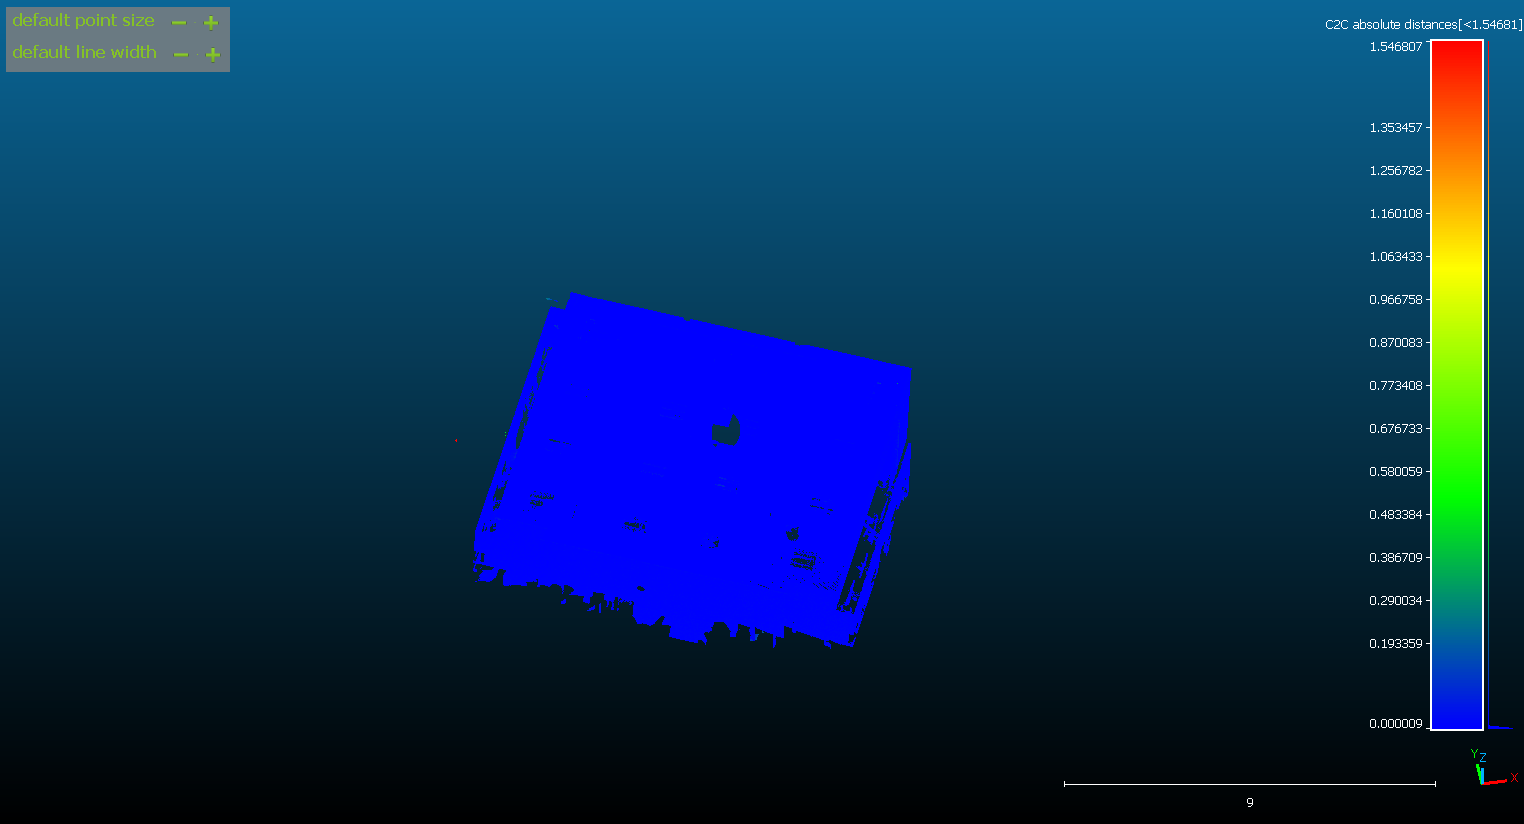
\includegraphics[height=\textheight/2 ,width=\textwidth/1]{figures/MLSasReference.png}
  \captionof{figure}{C2C Distance Visualization of MLS as the Reference Point Cloud}
  \label{fig:c2cMLS}
\end{minipage}

As seen in figure \ref{fig:c2cMLS} and table \ref{tab:RMStable2}, the areas in which there is only overlap between the TLS and MLS shows very high quality, where there are no outliers involved. This highlights how the TLS is not prone to many outliers. The distances between both point clouds are also on average, about 0.091cm, compared to the C2C distances when outliers were involved, as seen in table \ref{tab:RMStable}, where the means are about 9cm for the area where all distances were considered. This difference could thus be explained by the outliers inflating the means.

To further investigate these distances, a histogram of the C2C distance was created from the saved text file of the MLS. Figure \ref{fig:c2chistogram} shows the histogram for C2C distances less than or equal to 1 and distances greater than 1. These distances are based on the initial C2C distance calculations in table \ref{tab:RMStable}.

\begin{minipage}{\linewidth}
  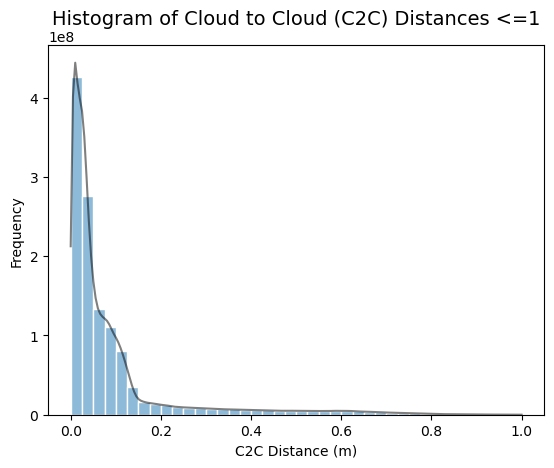
\includegraphics[height=\textheight/4 ,width=\textwidth/2]{figures/MLSC2CHistogramWithLine.png}
  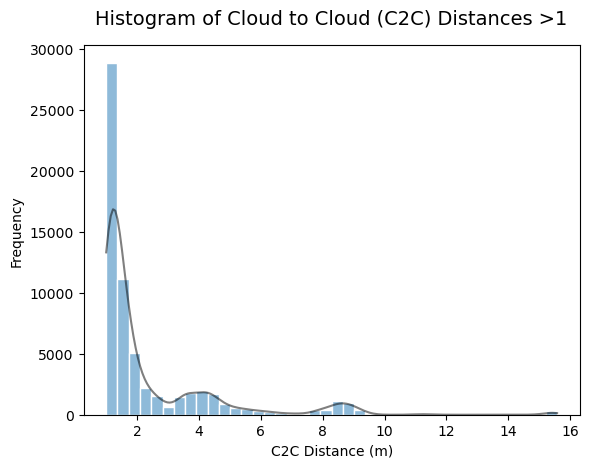
\includegraphics[height=\textheight/4 ,width=\textwidth/2]{figures/MLSC2CHistogramWithLine2.png}
  \captionof{figure}{Probability distribution of distances less than or equal to 1 (left) and distances higher than 1(right). Note that frequency for the left table is multiplied by \num{1e8}}
  \label{fig:c2chistogram}
\end{minipage}

The proportion of points that are less than 1 is much higher (99.93\% of the total point cloud) than points that are greater than 1 (0.00075\% of the total point cloud), as seen in table \ref{tab:RMStable}. For those with distances less than or equal to 1, the probability of points being less than 0.2 is much greater than the probability of a point being above 0.2, with most of the distances being close to 0, slowly reducing in frequency and eventually plateauing without any significant increase in frequencies. This indicates a high accuracy in the alignment and overlapping of both point clouds. This is also shown in figure \ref{fig:maxdistanceset}, where most of the overlapping areas of the TLS and MLS point clouds are coloured blue, indicating very close C2C distances for that area. 

Meanwhile, the probability distribution of points that have C2C distances greater than 1 show slightly more distribution. Similar to the C2C distances that are less than one, most of the C2C distances are clustered before 3. These points are representative of higher C2C distances found in figure \ref{fig:maxdistanceset} where red colours are surrounding the overlapping area of the point clouds. However, there are areas in which there is gross difference in the calculated distances, as seen in figure \ref{fig:grossError}. To investigate this, the significant increases after 3 C2C distance will be investigated.

There are significant increases occuring in the range of 3-5 and 9-10. Looking at figure \ref{fig:nomaxdistance}, there are areas where the MLS point cloud drifts away from the TLS point cloud, which are shown in green. A visualization of the areas described with large C2C distances are shown in figure \ref{fig:grossError}. The scale indicates green starting at about 3 C2C distances and ending at about 7.7 C2C distances. This would explain the frequency increase seen in the histogram. However, this increase goes back down in the histogram. Again looking at figure \ref{fig:grossError}, there is a section in which the MLS point cloud extends from the TLS point cloud, before there being a large amount of empty space, followed by further errors shown. These errors are indicated in red, which range from 11-15 C2C distances. This would explain why the histogram shows an increase in the 3-5 range, before going back down and coming back up at the 9-10 range, as these two error areas are separated by a significant of empty space. 

\begin{minipage}{\linewidth}
  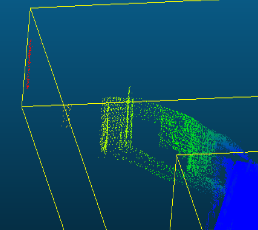
\includegraphics[height=\textheight/4 ,width=\textwidth/2]{figures/grossError.png}
  \captionof{figure}{Area With Large C2C Distances in the MLS Point Cloud}
  \label{fig:grossError}
\end{minipage}

These results show good accuracy in the alignment of the point clouds, as the C2C distances are mostly low (99.5\% being under 1, with most of these point being close to 0). For the area in which C2C distances are greated than 1, these points are much less influential on the results due to their low proportion relative to the whole point cloud (0.00075\%). Furthermore, even within that 0.00075\%, the outliers in \ref{fig:grossError} make up an even smaller proportion of the point clouds, with most distances being in the 1-3 C2C distances range. The average C2C distances for points that are not gross outliers (less than 1), are also very low, with a mean of 0.09. Some areas of the point clouds also had distances of \num{1.4e-5}, which is very close to 0. The maximum error of points that were relevant to the area being modeled is also at 0.046, indicating a low error rate.

\subsection{Completeness of Point Clouds}

To investigate the completeness of each point cloud, figure \ref{fig:maxdistanceset} was investigated. Visual inspection shows that there are areas with high C2C distances, shown in red. Most of these points are areas in which there is no overlap with the TLS point cloud area, like those described when discussing the probability distribution above. These areas are likely due to a lack of correspondence and have no overlap with the area being modelled (the room). However, some areas show high C2C distances even when the area is overlapping. Particularly, on the flooring area of the building. To further investigate, the point clouds were subsampled, reducing the amount of points in each cloud. This allows an inspection of the inside of the room. These are shown in figure \ref{fig:subsampledareas}.

\begin{minipage}{\linewidth}
  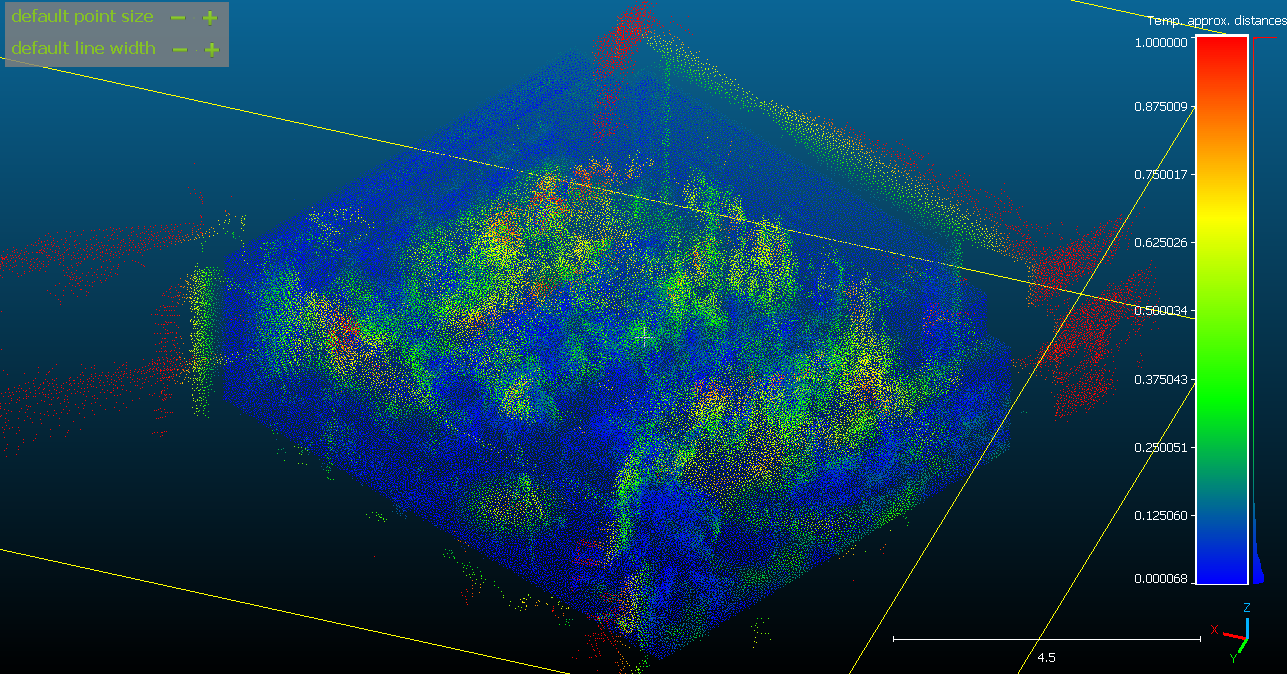
\includegraphics[height=\textheight/4 ,width=\textwidth/2]{figures/subsampledMLS.png}
  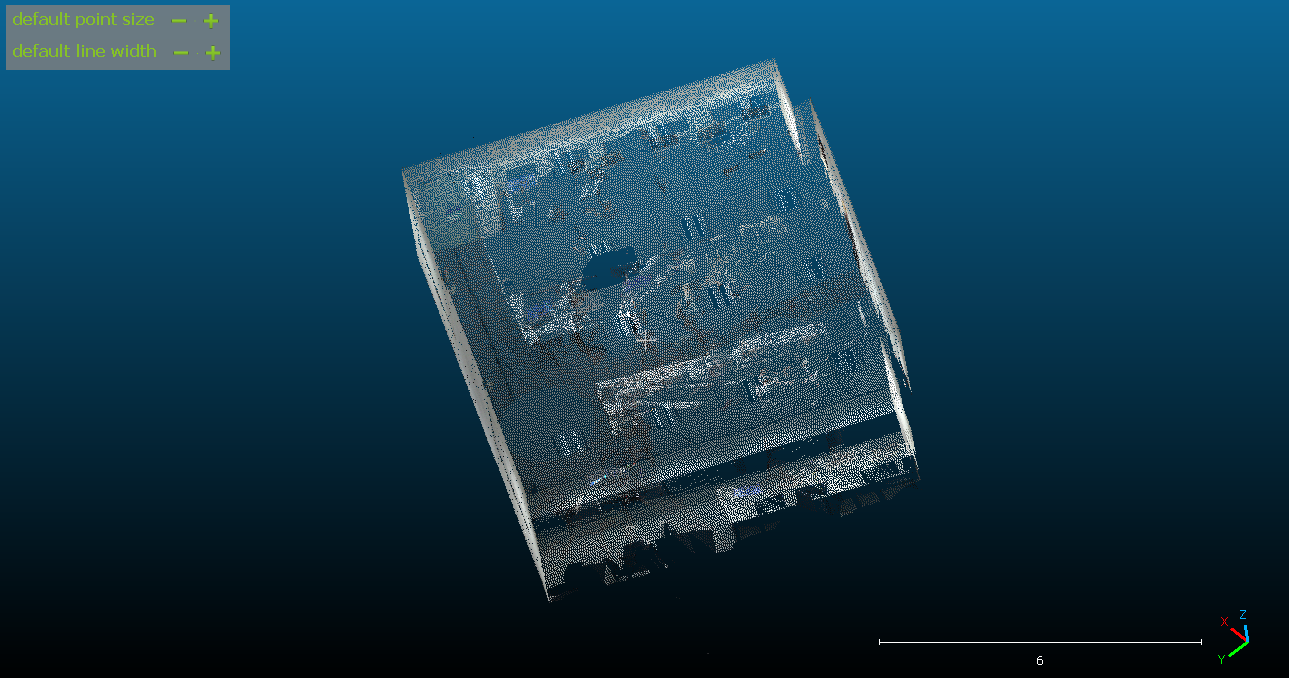
\includegraphics[height=\textheight/4 ,width=\textwidth/2]{figures/subsampledTLS.png}
  \captionof{figure}{Subsampled areas of the MLS (left) and the TLS (right) point clouds}
  \label{fig:subsampledareas}
\end{minipage}

The subsampling of the MLS shows that areas inside the room had a significant amount of high C2C distances, even when it was overlapping with the TLS point cloud. The TLS point cloud subsample could indicate why this was the case, as the flooring area of the room had a large area in which there are no points. This could be due to the position of the TLS apparatus and orientation of the room, which has a lot of objects blocking the TLS apparatus' field of view. To further investigate, a top-down view of the subsection of both MLS and TLS point clouds are shown in figure \ref{fig:subsectionedAreas}.

\begin{minipage}{\linewidth}
  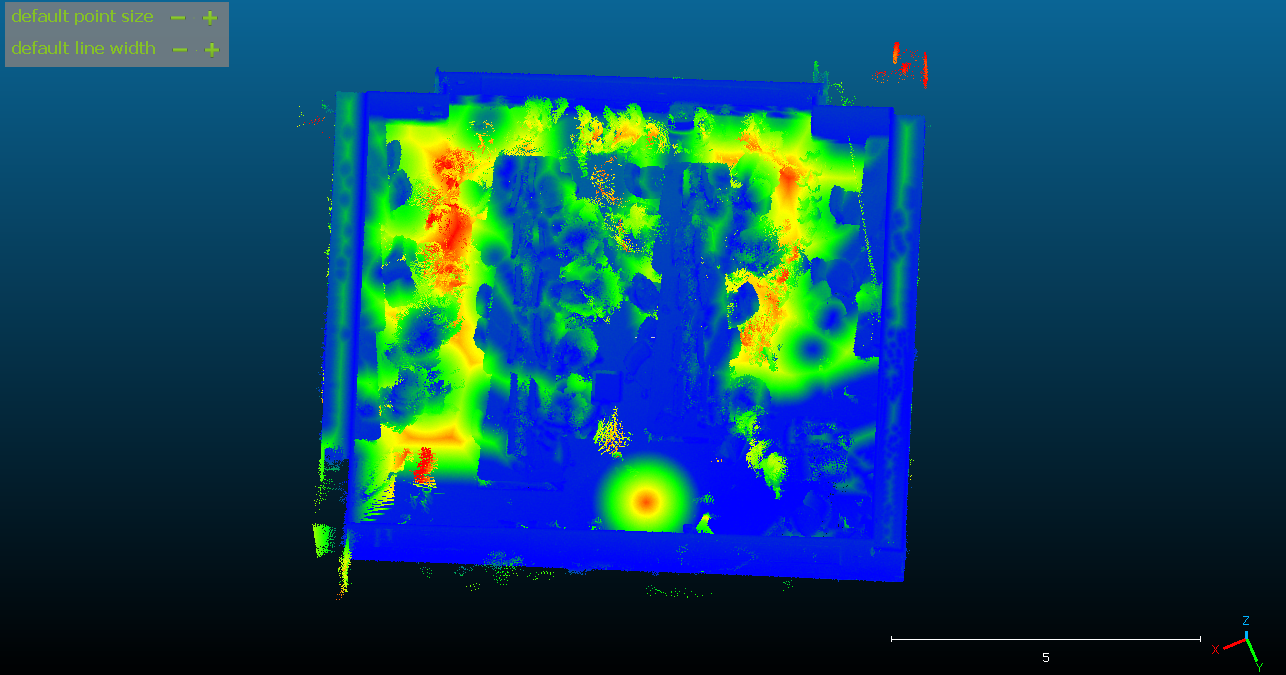
\includegraphics[height=\textheight/4 ,width=\textwidth/2]{figures/subsectionedMLS.png}
  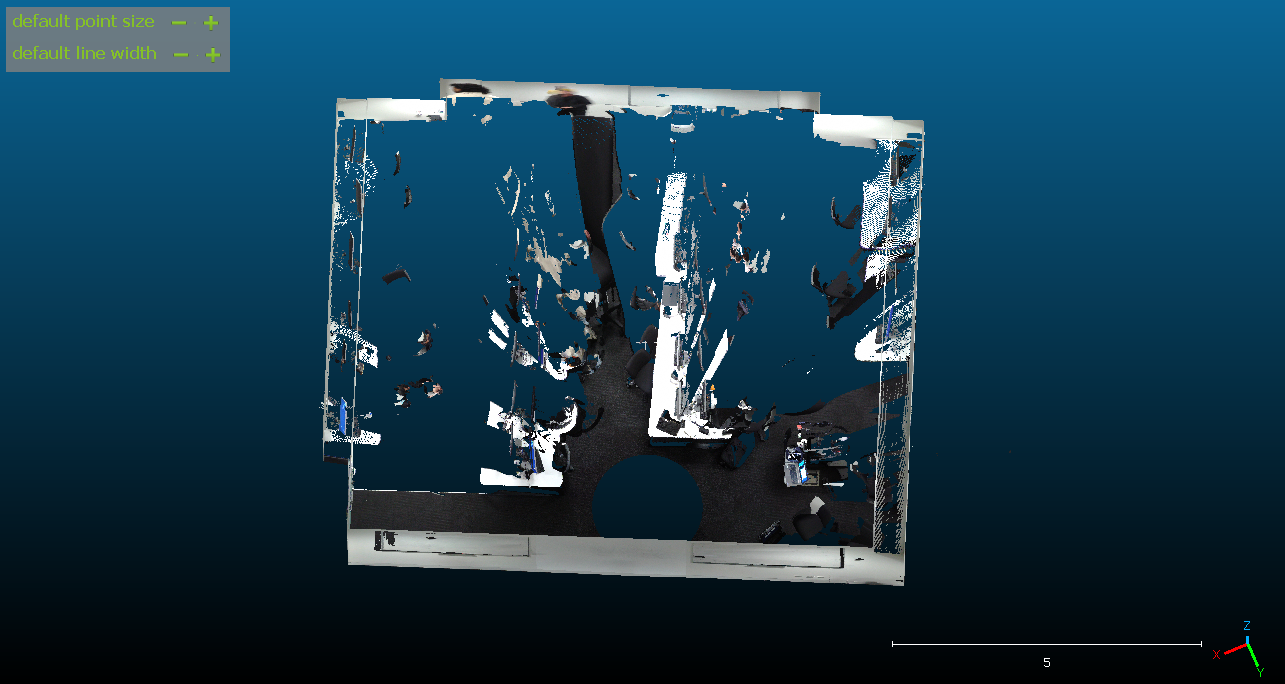
\includegraphics[height=\textheight/4 ,width=\textwidth/2]{figures/subsectionedTLS.png}
  \captionof{figure}{Subsectioned areas of the MLS (left) and the TLS (right) point clouds with a top-down view}
  \label{fig:subsectionedAreas}
\end{minipage}

The subsectioned areas show where the blindspots of the TLS apparatus are due to a blocked field of view (including under it, where the tripod was positioned). Mostly, these are found in the floors, explaining why in the TLS subsection in figure \ref{fig:subsectionedAreas} above has high C2C distances (ranging from green to red) \footnote{The MLS subsection was taken from the model in figure \ref{fig:maxdistanceset}}. This shows how in terms of completeness, TLS was unable to create a whole complete reconstruction of the room, while MLS was able to do this. This would make sense, as the MLS was moved around to capture every part of the room and if there was something blocking its field of view, the MLS apparatus could simply be moved around to capture around the blocked area, while the TLS needs to remain stationary. The completeness of the MLS however, also brings some disadvantages. To illustrate, figure \ref{fig:grossError} shows areas where there are point clouds much further away from the area trying to be modelled, and this is present only in the MLS point cloud.

While the field of view issue causes large C2C distances, it is not the only area in which there are large C2C distances. Some areas that have overlap in both TLS and MLS point clouds and not being hindered by the field of view blockage are shown to have green C2C distances (\ref{fig:subsectionedAreas}). This could be due to how the area being modelled was not being kept consistent (e.g., people were moving around). This causes inconsistent point cloud generatoin, and thus increased C2C distances in these areas. This shows that the point cloud might be complete in some areas for both TLS and MLS point clouds, but the inconsistent environment leads to increased C2C distances.

Another point to make regarding completeness is that TLS is able to capture images in colour, while the MLS only shows the density of points and intensity obtained in the area, as seen when the images were first placed into CloudCompare (figure \ref{fig:manualAlignment}). In this sense, TLS is more "complete" as it captures more information regarding the area being modelled, that is the colours of the room. Furthermore, neither MLS or TLS were able to capture the exterior of the building. This is more obvious for the TLS, as seen in figure \ref{fig:exteriorArea}.

\begin{minipage}{\linewidth}
  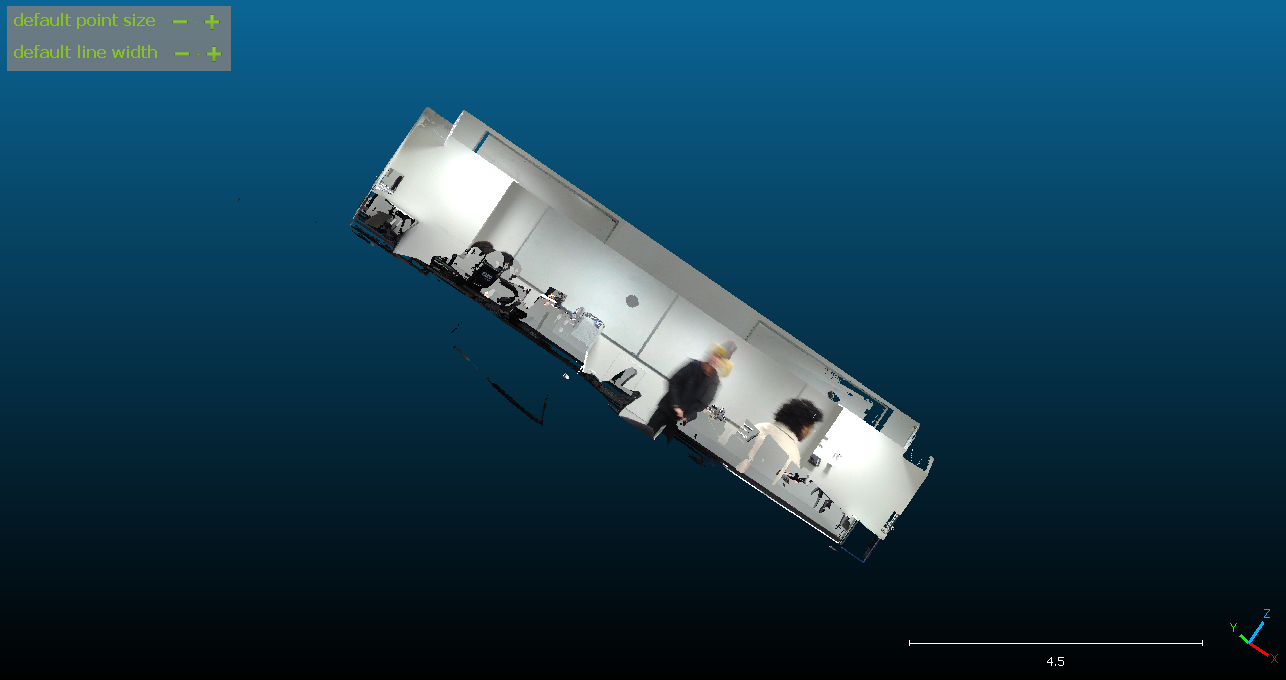
\includegraphics[height=\textheight/4 ,width=\textwidth/2]{figures/exteriorTLS.png}
  \captionof{figure}{Exterior View of A Wall in the TLS Point Cloud}
  \label{fig:exteriorArea}
\end{minipage}

The exterior walls of the TLS point cloud are shown to have textures of things inside the room, such as the people walking around. This is due to how the TLS also captures colours. As for the MLS, it would not have this problem as it was not capturing colours. However, the shape of the exterior would still not be completely accurate. In short, it could be summarised as the TLS not being able to capture both the shape and colour of exteriors, while the MLS is unable to capture only the shape as it doesnt capture colours. 

In conclusion, MLS can generally be considered more complete as it covers a more complete area, albeit at the risk of getting outliers. TLS, while it has less coverage and thus less completeness, can capture colours of the area being scanned. However, both MLS and TLS are not able to capture exterior shapes due to the physical limitations of the apparatus and the space.

\section{Conclusion and Discussion}

In this report, I have successfully compared two point clouds from a MLS and TLS apparatus. I have showed the RMS errors resulting fro alignment of both point clouds, as well as the C2C distances and compared the completeness. Overall, the comparison of the point clouds show good accuracy (with RMSE of fine registration being 2.27cm total). In addition, the C2C distances display low C2C distances dominating the distributions shown in \ref{fig:c2chistogram}. 

However, certain areas still show low quality of point cloud registration, particularly the outliers in the MLS point cloud and the blind spots in the TLS. \Textcite{conti2024} suggested that TLS is better for higher quality and detailed modelling, while MLS provides a better and more efficient workflow. Based on my report, this is true, where TLS is able to capture colours and more details on objects (as seen in how the resulting point cloud is more interpretable as to what the room actually looks like). On the other hand, the MLS point cloud is difficult to distinguish what objects are which, as they do not capture colour. However, there are nuances that should be considered as well when talking about the use of each MLS and TLS. MLS was able to capture more areas without being limited by its blind spot, albeit at the cost of outliers. Meanwhile, TLS had a lot of blind spots that it could not capture, but it did not have many outliers and for the areas that it did capture, it captured with high quality. 

The issues described above show the way MLS and TLS can complement each other. MLS is able to have an efficient workflow where areas difficult to reach can be recorded and scanned. Meanwhile, TLS provide the high quality that a model might require. One example of how these two LiDAR methods can be used together is suggested by \Textcite{Levick2021}, which performed a study on both MLS and TLS methods in mapping forestry. They suggested that the TLS could act as a calibration and validation tool for MLS. A similar approach to this calibration and validation with TLS is present in this report. In the context of this report, the MLS point cloud of the room was validated with the TLS, which resulted in the ability to identify outliers and which areas might tend to cause more errors. Using both also serves to decide which errors are acceptable and which erroneous point clouds could be removed. For instance, the floor not being scanned by the TLS would not be an issue if we were only using the MLS point cloud to perform imaging, but outliers caused by the MLS itself would have to be removed. Being able to identify the two was also a result of using the TLS to verify the MLS.

Furthermore, while the Hovermap Esement MLS is not able to capture colours, some other MLS apparatus have the capacity to capture colours, such as the Artec Leo (\Textcite{artecleo}), these are generally very expensive, but could provide an additional layer of verification and calibration by comparing the colours obtained from the MLS and the TLS. Nevertheless, MLS calibration by TLS for MLS cloud points without colours still has its place. For example, the government of Western Australia released a MLS scanning standard for its roads (\Textcite{scanningStandard}). This manual states that "RGB colour point cloud is not required for Design Grade and Concept Grade MLS", showing that even in real life-applications, MLS without colours can still be calibrated with TLS to ensure prescision and identify and possible errors in scanning.

In conclusion, I have successfully compared MLS and TLS point clouds using CloudCompare, identifying possible outliers and errors as well as suggesting reasons for these errors (e.g., blind spot in TLS). I have also compared the quality of TLS and MLS scanning, showing that there are nuances on which to choose (e.g., choosing high quality models with the TLS or model areas that might have blind spots with the MLS). Furthermore, I have also suggested that using both TLS and MLS can allow for verification and evaluation of an MLS point cloud, allowing identification of error sources even if the TLS has blind spots (e.g., outliers caused by MLS or an acceptable error such as the errors caused by the missing floor).

\printbibliography

\newpage

\section{Appendix}
Appendix A - Obtaining Max Error for Maximum Distances of About 1

To obtain the max errors, the subsectioning was done to remove outlying points, as shown in \ref{fig:subsectionSample}. This causes more \% of the points between the TLS and MLS to overlap for the distance calculations. The two subsectioned areas then went a C2C distance calculation like those described in the Cloud to Cloud Distance in the methodolgy section. The resulting maximum error was then noted, as shown in figure \ref{fig:subsectionResults} The initial results (all of the points being used for C2C Distance also showed a resulting section like those in figure \ref{fig:subsectionResults}).

\begin{minipage}{\linewidth}
  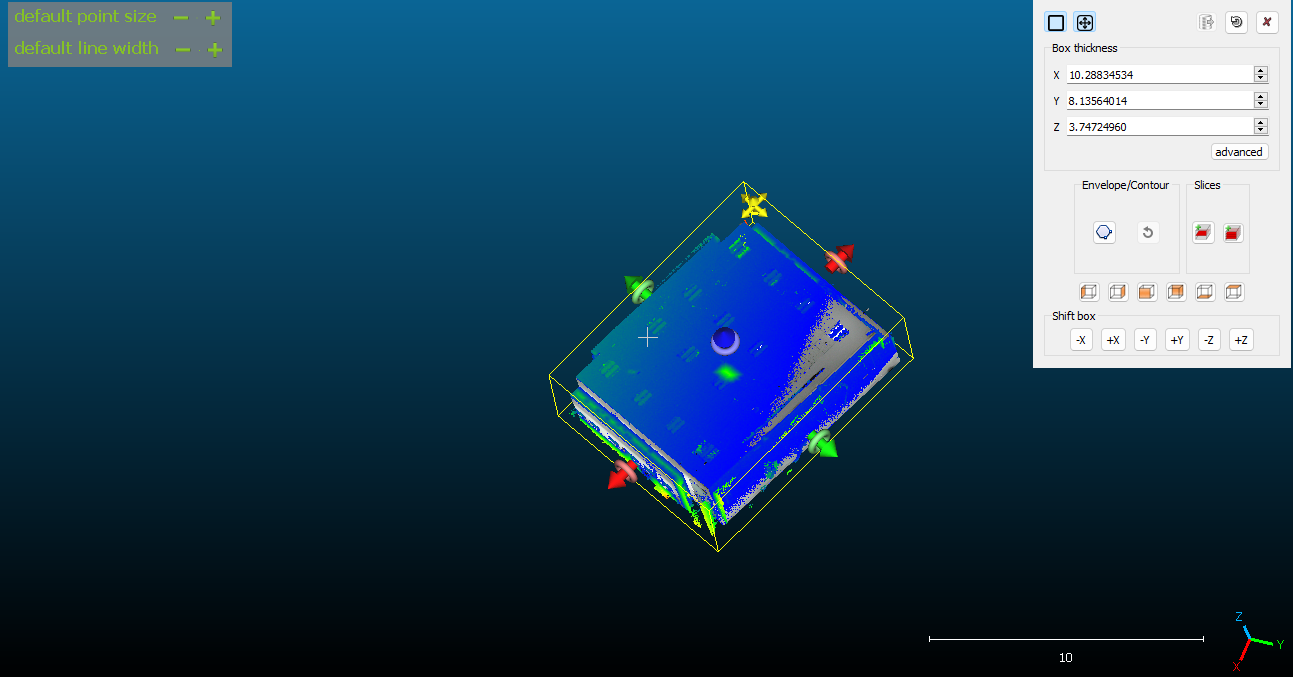
\includegraphics[height=\textheight/6 ,width=\textwidth/2]{figures/exampleSubsectioning.png}
  \captionof{figure}{Process of Subsectioning}
  \label{fig:subsectionSample}
\end{minipage}

\begin{minipage}{\linewidth}
  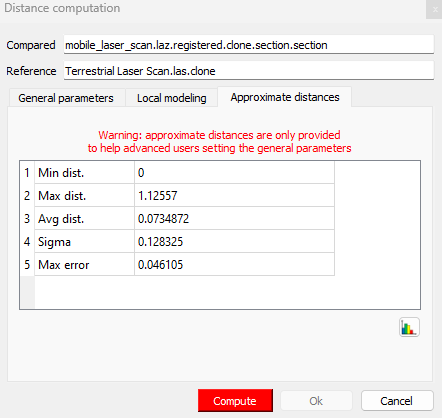
\includegraphics[height=\textheight/4 ,width=\textwidth/2]{figures/exampleSubsectioning2.png}
  \captionof{figure}{Results of C2C Distance Calculations After Subsectioning the MLS}
  \label{fig:subsectionResults}
\end{minipage}



\end{document}
